% This file was created with matplot2tikz v0.4.0.
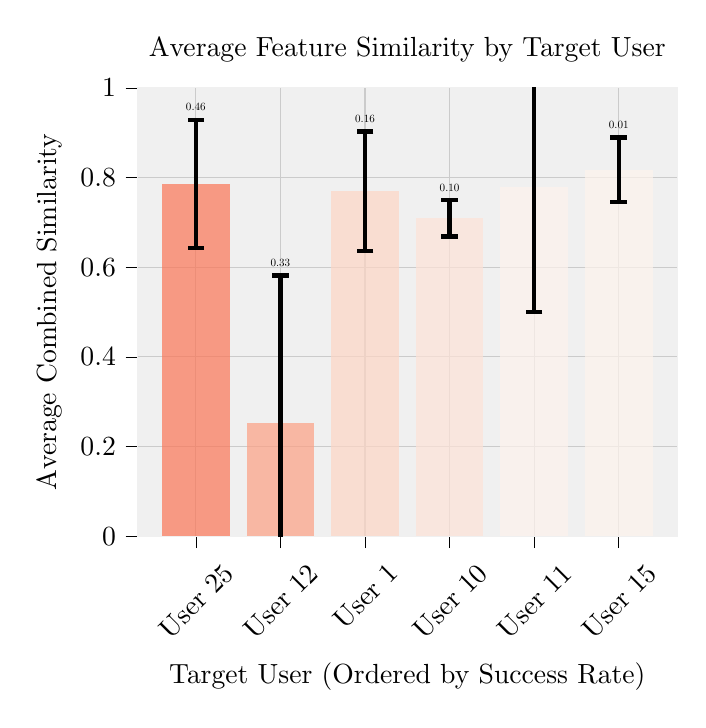
\begin{tikzpicture}

\definecolor{antiquewhite254227215}{RGB}{254,227,215}
\definecolor{coral25111785}{RGB}{251,117,85}
\definecolor{lightgray203}{RGB}{203,203,203}
\definecolor{lightsalmon252160131}{RGB}{252,160,131}
\definecolor{peachpuff253214197}{RGB}{253,214,197}
\definecolor{seashell254242236}{RGB}{254,242,236}
\definecolor{seashell254243237}{RGB}{254,243,237}
\definecolor{whitesmoke240}{RGB}{240,240,240}

\begin{axis}[
axis background/.style={fill=whitesmoke240},
axis line style={whitesmoke240},
tick align=outside,
tick pos=left,
title={Average Feature Similarity by Target User},
x grid style={lightgray203},
xlabel={Target User (Ordered by Success Rate)},
xmajorgrids,
xmin=-0.69, xmax=5.69,
xtick style={color=black},
xtick={0,1,2,3,4,5},
xticklabel style={rotate=45.0},
xticklabels={User 25,User 12,User 1,User 10,User 11,User 15},
y grid style={lightgray203},
ylabel={Average Combined Similarity},
ymajorgrids,
ymin=0, ymax=1,
ytick style={color=black}
]
\draw[draw=none,fill=coral25111785,fill opacity=0.7,very thin] (axis cs:-0.4,0) rectangle (axis cs:0.4,0.785773415840267);
\draw[draw=none,fill=lightsalmon252160131,fill opacity=0.7,very thin] (axis cs:0.6,0) rectangle (axis cs:1.4,0.252969630132856);
\draw[draw=none,fill=peachpuff253214197,fill opacity=0.7,very thin] (axis cs:1.6,0) rectangle (axis cs:2.4,0.769479632252265);
\draw[draw=none,fill=antiquewhite254227215,fill opacity=0.7,very thin] (axis cs:2.6,0) rectangle (axis cs:3.4,0.708889005897983);
\draw[draw=none,fill=seashell254242236,fill opacity=0.7,very thin] (axis cs:3.6,0) rectangle (axis cs:4.4,0.77899848360508);
\draw[draw=none,fill=seashell254243237,fill opacity=0.7,very thin] (axis cs:4.6,0) rectangle (axis cs:5.4,0.817470183239012);
\path [draw=black, ultra thick]
(axis cs:0,0.643024625957353)
--(axis cs:0,0.92852220572318);

\path [draw=black, ultra thick]
(axis cs:1,-0.0754832225124567)
--(axis cs:1,0.581422482778168);

\path [draw=black, ultra thick]
(axis cs:2,0.636698260109759)
--(axis cs:2,0.902261004394771);

\path [draw=black, ultra thick]
(axis cs:3,0.668313293589871)
--(axis cs:3,0.749464718206095);

\path [draw=black, ultra thick]
(axis cs:4,0.499919049479051)
--(axis cs:4,1.05807791773111);

\path [draw=black, ultra thick]
(axis cs:5,0.745848250009592)
--(axis cs:5,0.889092116468432);

\addplot [ultra thick, black, mark=-, mark size=3, mark options={solid}, only marks]
table {%
0 0.643024625957353
1 -0.0754832225124567
2 0.636698260109759
3 0.668313293589871
4 0.499919049479051
5 0.745848250009592
};
\addplot [ultra thick, black, mark=-, mark size=3, mark options={solid}, only marks]
table {%
0 0.92852220572318
1 0.581422482778168
2 0.902261004394771
3 0.749464718206095
4 1.05807791773111
5 0.889092116468432
};
\draw (axis cs:0,0.94852220572318) node[
  scale=0.4,
  anchor=base,
  text=black,
  rotate=0.0
]{0.46};
\draw (axis cs:1,0.601422482778168) node[
  scale=0.4,
  anchor=base,
  text=black,
  rotate=0.0
]{0.33};
\draw (axis cs:2,0.922261004394771) node[
  scale=0.4,
  anchor=base,
  text=black,
  rotate=0.0
]{0.16};
\draw (axis cs:3,0.769464718206095) node[
  scale=0.4,
  anchor=base,
  text=black,
  rotate=0.0
]{0.10};
\draw (axis cs:4,1.07807791773111) node[
  scale=0.4,
  anchor=base,
  text=black,
  rotate=0.0
]{0.02};
\draw (axis cs:5,0.909092116468432) node[
  scale=0.4,
  anchor=base,
  text=black,
  rotate=0.0
]{0.01};
\end{axis}

\end{tikzpicture}
